% Generated by scripts/supp_tex.py from scripts/supp/f_router.py.
% Do not edit: edit the module, which also builds the PDF version.

\section{The router and the calibrated bit rule}
\label{supp:f_router}

An exit map assigns one exit index to every tile of a frame, and this work produces one in three ways. Configuration A searches all K exits for every tile at the encoder, which holds the source, and signals the answer. Configuration B predicts the map at the decoder from data the decoder already holds, and signals nothing. The third way computes it at the decoder from one number the entropy coder has already produced, with nothing learned. The main paper states the rule by which the head turns logits into an exit and where its tilt comes from, and that is not repeated. What is here is the head itself, what each of its inputs is worth, what it costs to run, and how it fares against the third way.

Write D(t,k) for the mean squared error of tile t decoded at exit k and c$_{k}$ for the cost of exit k in units of one released decode. At a price \lambda on compute, the Lagrangian oracle gives each tile the exit that minimises

\begin{equation}
\ell(t,k) \;=\; D(t,k) \,+\, \lambda\, c_k, \qquad k^{*}(t) \;=\; \mathrm{arg\,min}_{\,k \geq j}\ \ell(t,k).
\end{equation}

The split depth j is the number of trunk groups every tile runs before any tile may leave, so exits below j do not exist and the minimisation starts there. Throughout this section, \emph{agreement} means the fraction of tiles on which a predictor picks the same exit as this oracle at the same \lambda. It is the quantity the head is trained on. Part of what F.4 reports is that it is not the quantity that decides which allocation is cheaper.

\subsection{What each input is worth}

The head reads four per-tile signals and one per-frame signal. Since F.4 finds that a rule reading a single number beats it, it is fair to ask which of the five carries anything. The ablation trains the same head once per input group, with every other group zeroed after its projection rather than deleted. Architecture, parameter count, optimiser, seed, image order and quality draws are then identical across the six runs, and the only thing that differs is how much the head is allowed to know. All six carry 148,176 parameters, which is the deployed head's 144,024 plus the projection for the bit count that the deployed head does not use.

The quality index q stays live in every single-group run. It is one number per frame, identical for every tile in that frame, so it can say which operating point the decoder is at and cannot, even in principle, tell two tiles of one frame apart. Holding it live keeps the runs comparable on per-tile information alone. The run with q on its own is then the floor that choice implies, which is the agreement reachable with no per-tile information whatever.

\begin{table}[t]
\centering
\resizebox{\columnwidth}{!}{%
\begin{tabular}{lrrrr}
\toprule
live inputs & agreement & $\pm$ s.e. & last 250 & over floor \\
\midrule
stem,qp & 0.7750 & 0.0074 & 0.7607 & +0.2744 \\
stem,latent,scales,bits,qp & 0.7721 & 0.0075 & 0.7543 & +0.2715 \\
latent,qp & 0.7448 & 0.0080 & 0.7433 & +0.2442 \\
scales,qp & 0.7156 & 0.0083 & 0.7170 & +0.2150 \\
bits,qp & 0.6202 & 0.0091 & 0.6137 & +0.1196 \\
qp & 0.4923 & 0.0114 & 0.4900 & -0.0083 \\
\bottomrule
\end{tabular}}
\caption{\textbf{What each router input is worth.} Read the first column against the last: only the stem moves agreement far from what a single constant exit already achieves. Agreement with the oracle's exit choice on 1,200 frames and 4,800 tiles the head never trained on, with one standard error taken across frames rather than across tiles, since tiles of one image are not independent draws. \emph{last 250} is the running held-out agreement over the final 250 training steps, on 12 tiles a step, and confirms that the end-of-run measurement is not a fluctuation. \emph{over floor} is the margin over the best single constant exit, which scores 0.5006 on these tiles.}
\end{table}

{\small results/router\_ablation.json, and the six per-variant training records results/router\_ablation\_stem.json and its five siblings. All on the pinned checkpoint, all at \lambda = 1.3$\times$10$^{-5}$, all 3,000 steps from seed 0.}

\begin{figure}[t]
\centering
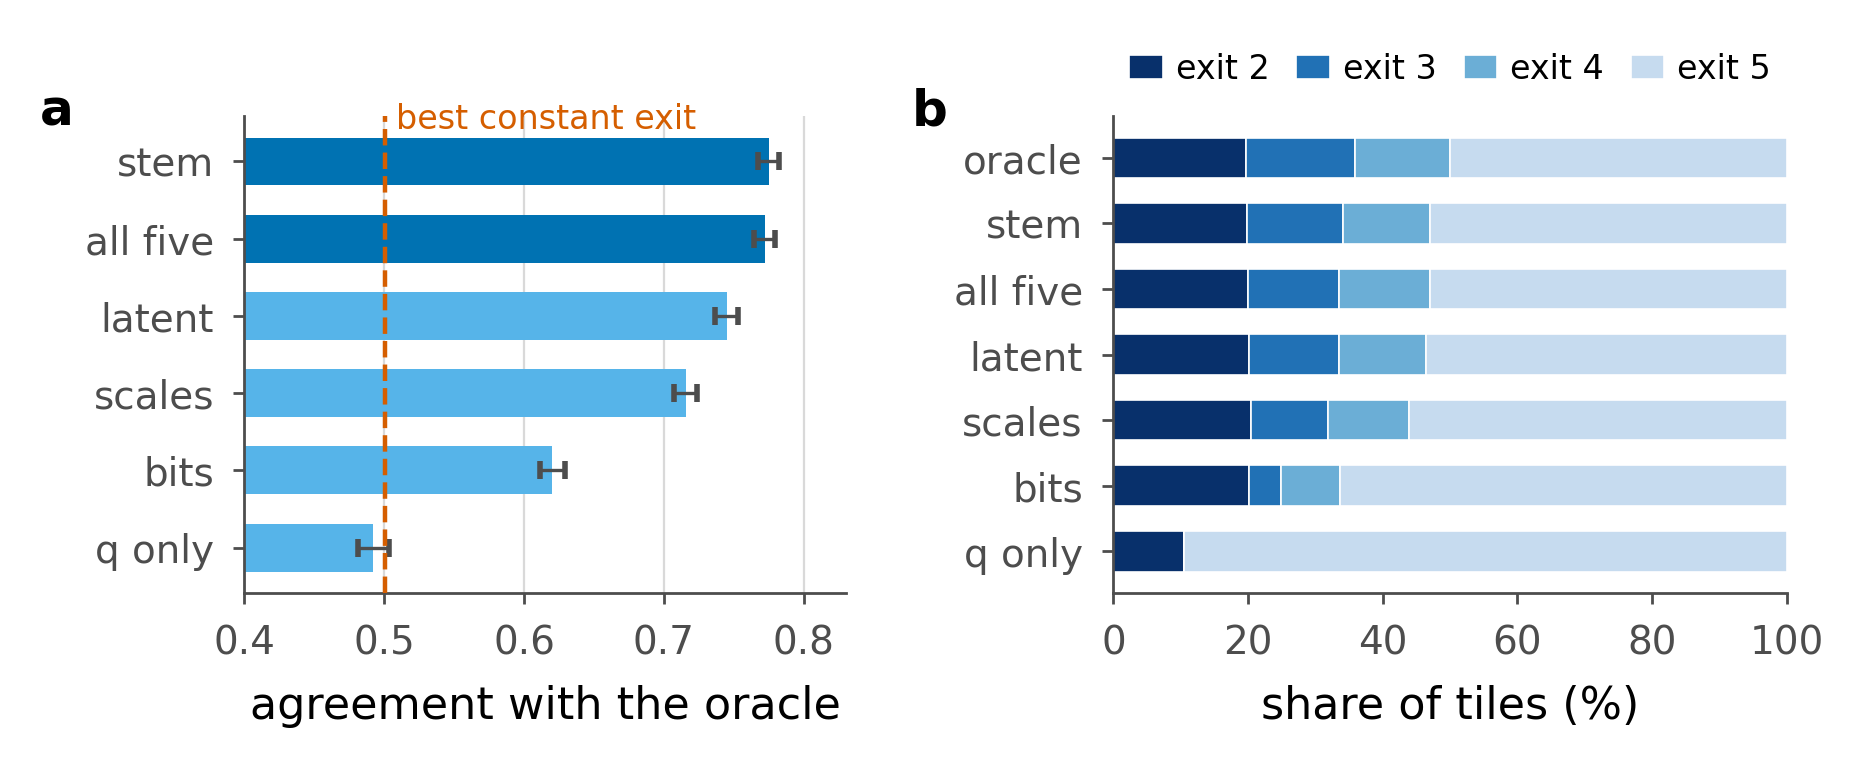
\includegraphics[width=\columnwidth]{figures/supp_router_inputs.png}
\caption{\textbf{The input ablation, both halves of it.} \textbf{a}, agreement with the oracle per variant, with one standard error across frames; the dashed line is the best single constant exit. The two dark bars are the two heads that see the stem. \textbf{b}, where each variant sends its tiles, against the oracle's own distribution. Every variant reproduces the oracle's use of the shallowest exit to within a point, and what degrades as inputs are removed is the separation of the middle of the ladder: the bit count alone nearly empties exit 3, and q alone uses two of the four exits available to it.}
\end{figure}

{\small Drawn by scripts/supp\_router\_figs.py from results/router\_ablation.json, fields agree, stderr, pred\_hist and oracle\_hist.}

\textbf{The stem alone.} Reading the stem and q gives 0.7750; reading the stem, the latent, the scales, the bit count and q gives 0.7721. The difference is 0.0029 against a standard error of 0.0105 on the difference, so it is under a third of one standard error and its sign is not determined. Four of the five inputs add nothing this measurement can resolve. That result is about those four inputs in this head, and it does not show that the latent, the scales or the bit count are uninformative about a tile. What it shows is that whatever they carry is already carried by the stem, which is computed downstream of all of them.

\textbf{The single-group ordering.} The stem at 0.7750 is 0.0302 above the latent, against a standard error of 0.0109 on the difference; the latent is 0.0292 above the scales; and the scales are 0.0954 above the bit count, which is more than seven standard errors. The bit count is the weakest per-tile input the head has, and F.4 shows a rule that reads the bit count and nothing else beating the head at every rate. The input the head learns least from is the input that wins when it is used differently.

\textbf{The floor.} The quality index on its own reaches 0.4923 $\pm$ 0.0114 where the best single constant exit scores 0.5006. A head with no per-tile information cannot beat the best constant in expectation, and this one does not. The floor belongs beside every other row, because an agreement of 0.62 cannot be read at all until it is known that 0.50 is free.

\textbf{The ablation's own cost.} The six trainings took 6.5 hours of one NVIDIA RTX A6000 between them, from 62 to 66 minutes each (results/router\_ablation\_*.json, field wall\_s). The decoder is frozen for all of them, so none of that is decoder training. It is the price of the question, and it is worth stating beside a negative answer.

One head covers every operating point, and the quality index is what makes that possible. It is an input rather than a selector: during training it is drawn uniformly at random for each batch, so one set of weights sees all 64 indices, and at test time the same weights run at every rate with the offline $\beta$ table of A.12 in front of them. No head per rate is proposed anywhere in this work, since that multiplies the stored parameters by the number of operating points a deployment offers, and F.5 is the measurement of what the single head gives up for that.

\subsection{What the head costs}

\begin{table}[t]
\centering
\resizebox{\columnwidth}{!}{%
\begin{tabular}{lrrrr}
\toprule
q & decode (ms) & stem (ms) & router (ms) & share (\%) \\
\midrule
0 & 114.29 & 41.25 & 0.571 & 0.500 \\
32 & 114.41 & 41.32 & 0.568 & 0.497 \\
63 & 114.44 & 41.31 & 0.568 & 0.496 \\
\bottomrule
\end{tabular}}
\caption{\textbf{The head against the decode it decides for.} The share column is the number to take away, and it is three times what the operation count predicts. Three timings on one latent, interleaved so that a co-tenant's load drift lands on all of them equally. \emph{decode} is the tiled decoder at the deepest exit, which is what the head's share is a share of; \emph{stem} is the first j groups, which the head does not pay for because the decoder runs them anyway before the split. The head takes \RouterTimePct\% of the decode where its operation count predicts \RouterCostPct\%, a factor of \RouterTimeFactor.}
\end{table}

{\small results/router\_latency.json: 1920$\times$1080 padded to 2048$\times$1280, 40 iterations after warm-up, one NVIDIA RTX A6000, the 144,024 parameter head runs/RECIPE512/routers2/v2\_lam1.3e-5.pth. Measured on runs/RECIPE512/ckpt\_eval.pth.tar rather than on the pinned checkpoint; the quantity is a ratio of two timings of the same weights, so it does not depend on which epoch they came from.}

The extra \RouterTimeExtra points are launch overhead. A head of 144,024 parameters evaluated on 40 vectors is small enough that its wall-clock is dominated by the cost of starting its kernels, and an operation count does not contain that. Every configuration-B saving in this work charges the head at its operation share, which is the smaller of the two numbers and therefore the more flattering to us; the honest reading is that the head costs about half a percent of the decode in time. It stays small against what it decides about, since one trunk block is 7.5\% of the decode by the cost vector below.

\textbf{Two heads, two shares.} The pinned checkpoint carries a head that was trained jointly with the decoder, and a second head was trained afterwards against that decoder once it was frozen. They are different objects and they are priced differently: the jointly trained one is charged 0.044\% of the decode and the frozen-decoder one \RouterCostPct\%, because the second reads the decoded latent and the entropy model's scales as well as the stem. Both shares are measured by hooks on the head's own convolutions and linear layers rather than assumed, in the same run that produced the saving. F.4 reports both heads.

{\small results/router\_RECIPE512\_b01\_jointhead.json and results/router\_RECIPE512\_b01.json, field router\_compute\_share\_pct in each.}

\textbf{For scale, what the search costs instead.} Configuration A does not run a head; it runs the argmin itself, which needs the true error of every exit, and section G prices that at 4.52 of a tiled decode per frame. A decoder-side head at half a percent of one decode, and a rule at nothing, are both several orders below it, which is the whole reason for wanting one.

\textbf{The head, exactly.} Three things enter. The first is the feature at the split point, 384 channels at one eighth of frame resolution, which is the last thing every tile shares. The second is the decoded latent concatenated with the entropy model's scales, the predicted Gaussian width used to code each latent position, which is already computed during the decode and is, position by position, an estimate of how hard that position was to code. The third is the quality index. Each of the first two is projected by a 1$\times$1 convolution, to 48 and 32 channels, then reduced to one vector per tile by taking the mean and the standard deviation over the tile. That gives 96 + 64 + 1 = 161 numbers per tile, which pass through a LayerNorm and a three-layer perceptron of width 256 with SiLU activations, ending in K logits. Almost all of the 144,024 parameters sit in the 1$\times$1 on the stem, which is the only part that runs per pixel; the perceptron runs once per tile, forty times for a 1080p frame, so its width is nearly free.

\begin{figure}[t]
\centering
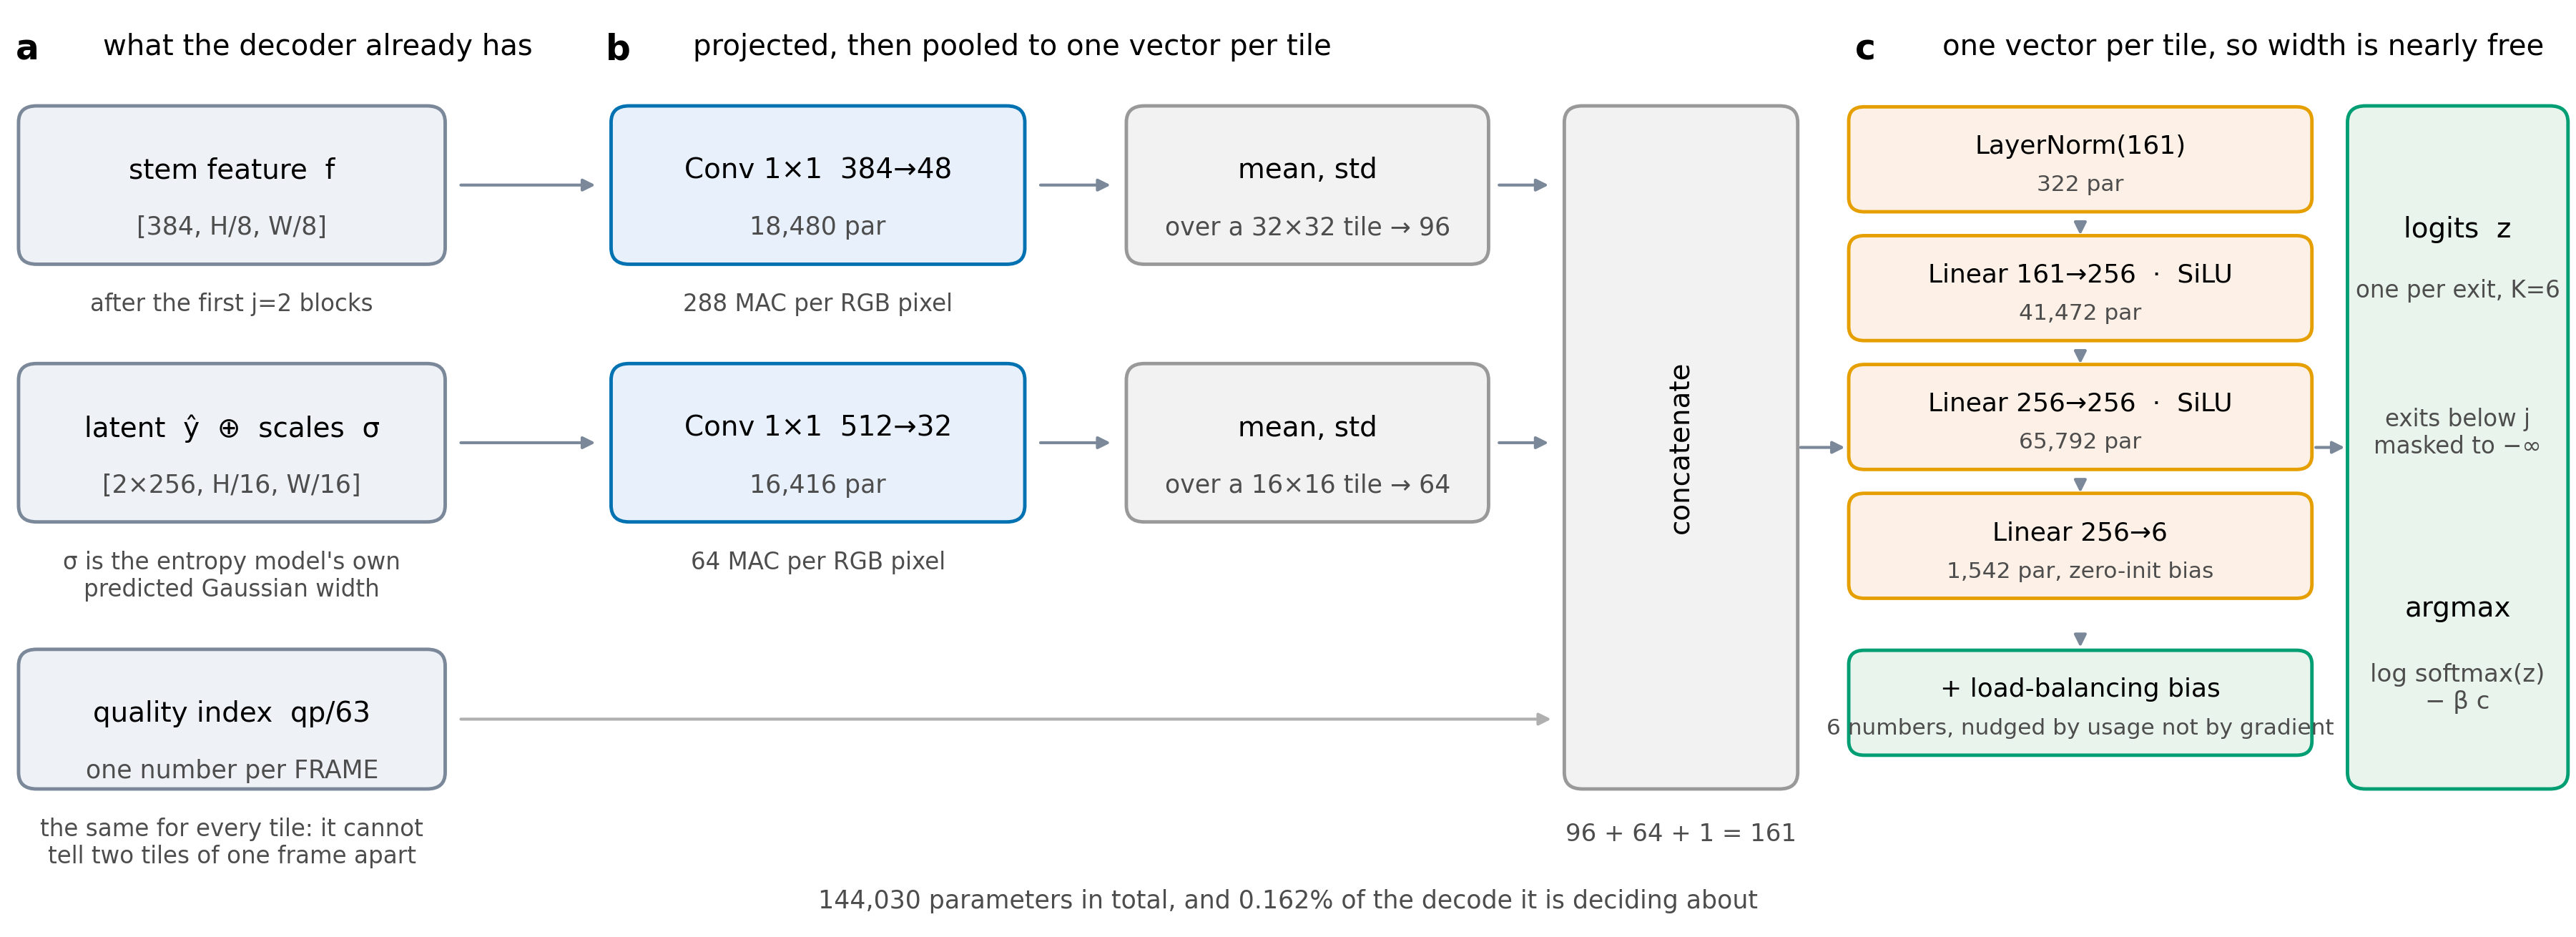
\includegraphics[width=\columnwidth]{figures/router_arch.png}
\caption{\textbf{The router head.} \textbf{a}, the three things it reads, all already held by the decoder at the moment the decision is needed. \textbf{b}, each projected by a 1$\times$1, then reduced to one vector per tile by its mean and standard deviation. \textbf{c}, a three-layer perceptron, one pass per tile. Every shape and parameter count in the figure is read off the module when the figure is drawn.}
\end{figure}

\textbf{What it is trained against.} The head is fitted against a frozen decoder, so the exits it chooses between do not move while it learns. Its target is the Lagrangian oracle's choice and the loss is a cross-entropy to that target, with each tile weighted by its \emph{regret}, meaning by how much the oracle's own bracket grows if the head's exit is used in place of the oracle's. A tile whose two best exits are nearly tied then counts for less than one where the wrong choice is expensive, which is the same asymmetry that makes agreement a poor score in F.4. A router of this shape can collapse onto a single exit during training, so it carries a balancing term: a per-exit bias added to the logits before the decision and updated by usage rather than by a gradient, which is what makes it loss-free [14]. It is biased toward the oracle's own exit distribution rather than toward uniform, because at a high multiplier the oracle genuinely does send every tile to one exit and forcing spread there would force mistakes.

\subsection{The calibrated bit rule}

The entropy model produces one number per tile before the trunk runs, at no cost, and then discards it: how many bits that tile's latents took. Per-block bit allocation is a standard quantity in learned compression, where it is something to choose, and block-level rate control sets it so that complex regions get more bits [40]. Here it is read in the other direction, after the fact and at the decoder, as a statement about how hard the region was. The results files call the rule \emph{rate-rank}; the paper calls it the calibrated bit rule. What follows is all of it.

\textbf{The statistic.} Sum the entropy coder's estimated bits r$_{i}$ over the latent positions i falling inside tile t, and divide by the mean over the N tiles of that frame. Normalising per frame rather than globally is deliberate: the absolute rate level is a property of the frame, and what decides a tile is how it compares with the rest of its own frame.

\begin{equation}
b(t) \;=\; N\, \frac{\sum_{i \in t} r_i}{\sum_{i} r_i}.
\end{equation}

\textbf{The surrogate.} Assume every tile has the same shape of decay across the ladder, up to a scale that depends only on b(t).

\begin{equation}
\log D(t,k) \;\approx\; \alpha \log b(t) \,+\, c \,+\, \log \varphi_k.
\end{equation}

$\varphi$ has one entry per reachable exit and says what that exit costs on an average tile; \alpha is an exponent fitted rather than assumed, which is what lets the rule find the direction of the relation instead of asserting one. The fit is offline and leave-one-sequence-out, so no sequence contributes to the profile that routes it, and its whole output is six numbers per rate.

\textbf{The decision.} Run the oracle's own Lagrangian on the surrogate table in place of the true one, and bisect \lambda against the budget as configuration A does.

\begin{equation}
\hat{k}(t) \;=\; \mathrm{arg\,min}_{\,k \geq j}\ \left[\, e^{c}\, b(t)^{\alpha}\, \varphi_k \,+\, \lambda\, c_k \,\right].
\end{equation}

\begin{table}[t]
\centering
\resizebox{\columnwidth}{!}{%
\begin{tabular}{l}
\toprule
\textbf{the decoder, once per frame} \\
\&nbsp;1\&nbsp; \emph{input} r, the entropy coder's estimated bits per latent position; the cost vector c; the price \lambda; the calibration (\alpha, c$_{0}$, $\varphi$) for this quality index \\
\&nbsp;2\&nbsp; \emph{for} each tile t of the N tiles of the frame \\
\&nbsp;3\&nbsp; \&nbsp;\&nbsp;\&nbsp;\&nbsp; b ← N $\cdot$ (sum of r$_{i}$ inside t) / (sum of r$_{i}$ over the frame) \\
\&nbsp;4\&nbsp; \&nbsp;\&nbsp;\&nbsp;\&nbsp; \emph{for} k = j … K$-$1 \\
\&nbsp;5\&nbsp; \&nbsp;\&nbsp;\&nbsp;\&nbsp;\&nbsp;\&nbsp;\&nbsp;\&nbsp; L$_{k}$ ← e$^{c$_{0}$}$ $\cdot$ b$^{\alpha}$ $\cdot$ $\varphi$$_{k}$ + \lambda $\cdot$ c$_{k}$ \\
\&nbsp;6\&nbsp; \&nbsp;\&nbsp;\&nbsp;\&nbsp; exit(t) ← the k that minimises L$_{k}$ \\
\&nbsp;7\&nbsp; \emph{return} exit \\
\textbf{offline, once per quality index, leave-one-sequence-out} \\
\&nbsp;8\&nbsp; d(t) ← mean over k $\geq$ j of log D(t,k) \\
\&nbsp;9\&nbsp; (\alpha, c$_{0}$) ← least squares of d(t) on log b(t) \\
10\&nbsp; log $\varphi$$_{k}$ ← mean over t of [ log D(t,k) $-$ \alpha log b(t) $-$ c$_{0}$ ] \\
\bottomrule
\end{tabular}}
\caption{\textbf{The calibrated bit rule, in full.} Lines 1 to 7 are what the decoder runs: one power and K products per tile, nothing learned, nothing signalled. Lines 8 to 10 are the offline calibration, whose entire output is the six numbers per rate printed in the next table. \lambda is bisected in two levels, on the cheap per-tile table first and then against a real decode of the resulting map, because the table and the decode differ slightly at the tile seams. Sweeping \lambda traces the lower convex hull of the achievable set in the sense of [26], so the point returned is the best one on that hull at the budget it consumes.}
\end{table}

\begin{table}[t]
\centering
\resizebox{\columnwidth}{!}{%
\begin{tabular}{lrrrrrr}
\toprule
q & delivered dB & \alpha & $\varphi$$_{2}$ & $\varphi$$_{3}$ & $\varphi$$_{4}$ & $\varphi$$_{5}$ \\
\midrule
0 & 0.1000 & 10.01 & 1.0216 & 0.9965 & 0.9932 & 0.9890 \\
16 & 0.1007 & 4.60 & 1.0229 & 0.9966 & 0.9930 & 0.9879 \\
32 & 0.1000 & 2.75 & 1.0262 & 0.9978 & 0.9910 & 0.9855 \\
48 & 0.1000 & 1.95 & 1.0282 & 0.9979 & 0.9902 & 0.9842 \\
63 & 0.0996 & 1.43 & 1.0302 & 0.9991 & 0.9882 & 0.9832 \\
\bottomrule
\end{tabular}}
\caption{\textbf{The rule's entire state}, at the 0.1 dB budget. There is nothing else to store, and it is printed here so that the rule can be reproduced without refitting it. \alpha is positive everywhere, so a tile whose latents cost more bits is modelled as harder at every exit and is sent deeper, which is what the correlations in F.4 confirm. $\varphi$ is nearly flat, spanning 3.3\% at q0 and 4.8\% at q63 between its shallowest and deepest entry, against costs that span 0.61 to 1.01, so what moves a tile along the ladder is its own b(t) rather than the shape of the profile. \emph{delivered dB} is what the two-level bisection actually landed on.}
\end{table}

{\small results/raterank\_RECIPE512\_b01.json, pinned checkpoint, \NumSeq CTC sequences at one frame each.}

The costs c$_{k}$ on the pinned checkpoint are 0.6088, 0.7578, 0.8697, 1.0095 for exits 2 to 5, recovered from the frame-level saving of maps that send every tile to one fixed exit. The shallowest of them, c\_j = 0.6088, sets the architectural ceiling of \CeilingModelled\%. The deepest is above 1 because our ladder carries seam repair and an adapter that the released decoder does not.

{\small results/static\_RECIPE512\_b01.json, field uniform, and results/saturation\_RECIPE512\_ctc53.json, fields cost\_j and ceiling\_pct.}

\subsection{The rule against the trained head}

Two trained heads exist on this checkpoint and both are reported, since averaging them would hide the only spread this work has. \emph{joint} is the head the checkpoint carries, trained alongside the decoder and read straight out of it. \emph{frozen} is the \RouterParams head trained afterwards, against the decoder once it had stopped moving. Both were evaluated on the pinned checkpoint over \NumSeq sequences at one frame each, by one script, at the same budgets, and both are charged for their own compute.

\begin{table}[t]
\centering
\resizebox{\columnwidth}{!}{%
\begin{tabular}{lrrrrrr}
\toprule
q & 0.1 rule & 0.1 joint & 0.1 frozen & 0.3 rule & 0.3 joint & 0.3 frozen \\
\midrule
0 & 34.48 & 26.84 & 28.96 & 39.12 & 39.08 & 38.96 \\
16 & 30.10 & 18.36 & 26.03 & 39.12 & 39.08 & 38.96 \\
32 & 24.90 & 13.21 & 23.00 & 39.12 & 39.08 & 38.96 \\
48 & 22.06 & 8.26 & 20.67 & 39.12 & 37.03 & 38.96 \\
63 & 20.14 & 5.13 & 18.49 & 39.12 & 34.07 & 38.96 \\
\bottomrule
\end{tabular}}
\caption{\textbf{The calibrated bit rule against two trained heads}, as the percentage of the released decoder's operations saved, at two budgets and five rates. The rule is ahead of both heads in every cell of this table. Every column is charged for what it costs: each head pays its own compute share and the rule pays nothing. The two heads are further apart from each other than either is from the rule at several rates, which F.5 takes up.}
\end{table}

{\small Rule: results/raterank\_RECIPE512\_b01.json and b03. Joint head: results/router\_RECIPE512\_b01\_jointhead.json and its b03 sibling. Frozen head: results/router\_RECIPE512\_b01.json and b03. All on runs/RECIPE512/ckpt\_PAPER.pth.tar.}

\begin{figure}[t]
\centering
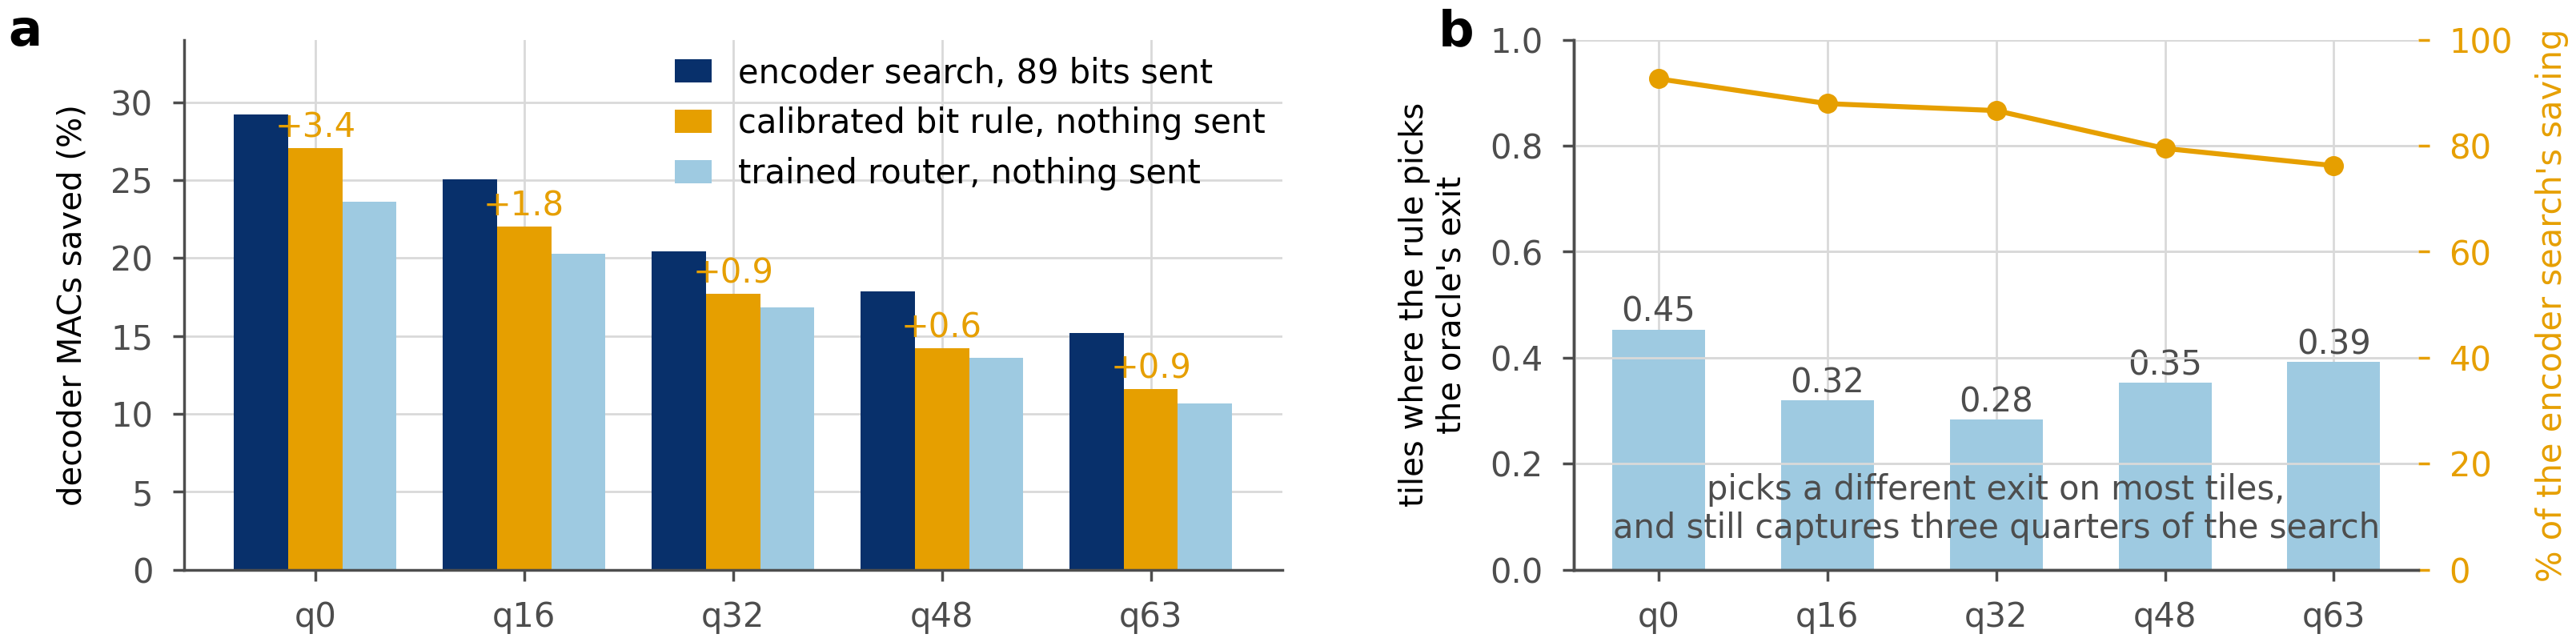
\includegraphics[width=\columnwidth]{figures/deciders.png}
\caption{\textbf{Three ways to choose an exit.} \textbf{a}, saving at 0.1 dB. The encoder search sees the source and sends 89 bits a frame; the other two send nothing. The bit rule beats the trained head at every rate, with no learned parameters against the head's 144,030. \textbf{b}, bars are the tiles where the rule picks the search's exit, the line the fraction of its saving it captures anyway. }
\end{figure}

\begin{figure}[t]
\centering
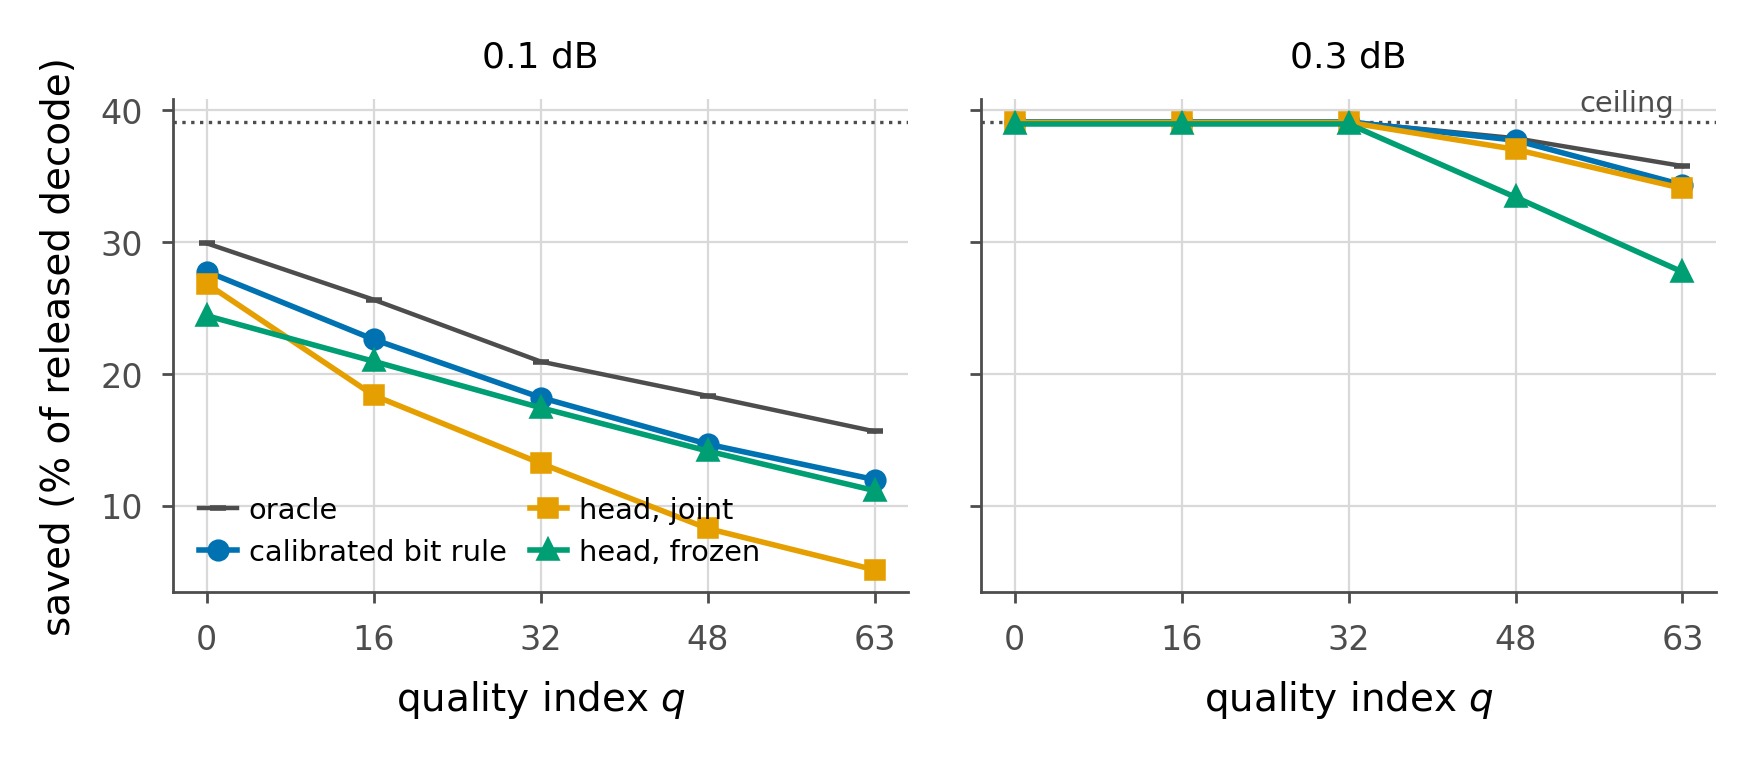
\includegraphics[width=\columnwidth]{figures/supp_router_frontier.png}
\caption{\textbf{The rule sits between the two heads and the oracle.} Saving at each rate, against the Lagrangian oracle measured inside the same run and the architectural ceiling (dotted). At 0.1 dB the rule is above both heads at every rate, and the gap between the two heads is wider than the gap between the rule and either of them. At 0.3 dB the three lowest rates saturate and the three curves separate only at q48 and q63.}
\end{figure}

{\small Drawn by scripts/supp\_router\_figs.py from the six files named in the table above and results/saturation\_RECIPE512\_ctc53.json.}

\textbf{At the working budget.} Against the joint head the rule is ahead by +7.65 points at its narrowest and +15.02 at its widest, the latter at q63. Against the frozen head it is ahead by +1.39 to +5.53 points. The rule reaches \RateRankLow\% at q0 and \RateRankHigh\% at q63, and it is ahead at all \RateRankNWins measured rates whichever head it is measured against. A head trained on this decoder against this oracle returns nothing over a rule with no learned parameters, while carrying a compute share that the rule does not.

\textbf{At 0.3 dB the low rates saturate and the arithmetic is exact.} At q0, q16 and q32 all three configurations send every tile to the shallowest exit, so the maps are identical and the only difference left is the price of deciding. The joint head falls 0.044 points below the \CeilingModelled\% ceiling and the frozen head 0.163, which are their compute shares of 0.044\% and 0.163\% to three decimals. At q48 and q63 the budget still binds and the allocations separate: the rule reaches 39.1\% and \RateRankLoose\% against the joint head's 37.0\% and 34.1\% and the frozen head's 39.0\% and 39.0\%. A looser budget gives an allocation more room to be wrong in as well as more room to be right, and the frozen head uses it to be wrong.

\textbf{Why 0.5 dB is not in that table.} At 0.5 dB every rate saturates for every configuration, so all three maps are identical and the only thing a comparison could measure is the cost vector each file was written with. The rule's 0.5 dB file is on runs/RECIPE512/ckpt\_eval.pth.tar, where the shallowest exit was priced at 0.6088 against the pinned 0.6088, a difference worth -0.00 points of apparent saving. The file is results/raterank\_RECIPE512\_b05.json and it records that the rule matches the oracle map exactly at all five rates there, which is the only thing read from it.

\begin{table}[t]
\centering
\resizebox{\columnwidth}{!}{%
\begin{tabular}{lrrrrr}
\toprule
q & rule agrees & $\rho$ depth & $\rho$ level & $\rho$ spread & oracle \\
\midrule
0 & 0.666 & +0.41 & +0.83 & +0.61 & 34.46 \\
16 & 0.462 & +0.45 & +0.85 & +0.68 & 30.83 \\
32 & 0.302 & +0.47 & +0.86 & +0.73 & 26.70 \\
48 & 0.237 & +0.51 & +0.84 & +0.80 & 25.38 \\
63 & 0.303 & +0.45 & +0.88 & +0.71 & 24.10 \\
\bottomrule
\end{tabular}}
\caption{\textbf{Why the rule works, and it is not by agreeing}, at 0.1 dB. Compare the second column with the fifth: the rule picks the oracle's exit on a minority of tiles and still tracks the oracle's saving. The three Spearman correlations are between a tile's bit count and, respectively, the depth the oracle assigns it, its mean distortion across the ladder, and the spread between its shallowest and its deepest exit. \emph{oracle} is the Lagrangian oracle measured inside the same run, which is the ceiling the rule is chasing.}
\end{table}

{\small results/raterank\_RECIPE512\_b01.json. The file stores spearman\_bits\_vs\_exit against the negated exit index, as scripts/raterank\_curve.py computes it, so the correlation with depth quoted here is its negative. The oracle column is measured at one frame per sequence and is not charged for the exit map; deployed configuration A, which carries the map, reads 34.5, 30.8, 26.7, 25.4, 24.1\% over the same five rates at two frames per sequence (results/signalled\_RECIPE512\_ctc53.json).}

The rule agrees with the oracle on \RateRankAgreeLo to \RateRankAgreeHi of tiles, well under the frozen head's held-out \RetrainAgreeOld, and saves more at every rate. Agreement counts a disagreement between two exits that are within a hair of each other exactly as heavily as one that costs most of the frame's error, and most disagreements are of the first kind. What the rule gets right is the ordering. A tile's bit count correlates with the spread across the ladder, which is how much that tile stands to gain from depth, at \RateRankSpreadLo to \RateRankSpreadHi at every rate, and with the depth the oracle actually assigns at +0.41 to +0.51.

What the rule cannot do is see past that ordering. A rank-1 model gives every tile the same relative profile over exits, so b(t) decides where on the ladder a tile falls and never the shape of its trade-off. That is the ceiling this baseline sits at, and it is the part a learned head would have to earn its parameters on. Neither of our two heads does.

\textbf{The two decoder-side signals are not complementary.} Normalising both surrogates to unit mean and blending them with one weight, from the calibrated bit rule at one end to the head's ordering at the other, the rule alone is best at every rate, and every positive weight is worse than none. Trusting the head completely costs \BlendCostMin to \BlendCostMax points, the most at \BlendCostMaxQ. The head reads the entropy model's scales and the bit count is what those scales produce, so blending them mixes a signal with a learned approximation of itself.

An earlier version of this table, measured before the checkpoint was pinned, showed a small gain at the two highest rates, and the paper carried it as evidence of weak complementarity. Re-measuring on the pinned weights removed it. The head in that measurement had been trained against whichever weights runs/RECIPE512/ckpt\_eval.pth.tar held at the time, which is a moving pointer, so the first suspicion was that the head had simply been measured against the weights it was fitted to. It had not. Repeating the sweep on the epoch-1 pin with the corrected cost model gives w=0 at every rate as well (results/combined\_RECIPE512\_b01\_e1.json), so the absence of complementarity survives a change of checkpoint and the gain was never a property of the two signals. What did change between the two measurements is the cost model: the earlier file predates the correction to the exit adapter's cost, and under the wrong cost an exit assignment can be scored better than it is. Every router number in this document is measured on the pinned checkpoint, after that correction, for this reason.

The same control makes a second point in passing. At w=0 the epoch-1 ladder saves more than the epoch-0 one at every rate -- 30.0 against 34.4 at q0 and 13.8 against 20.2 at q63 -- which is the epoch series of Section 5 seen through a different measurement. The checkpoint the paper reports is the first one, and it is the weakest one we have.

\begin{table}[t]
\centering
\resizebox{\columnwidth}{!}{\begin{tabular}{lrrrrrrr}
\toprule
$q$ & bits & 0.1 & 0.25 & 0.5 & 0.75 & 0.9 & head \\
\midrule
0 & \textbf{29.8} & 27.9 & 27.9 & 27.9 & 28.0 & 27.9 & 28.0 \\
16 & \textbf{24.1} & 23.3 & 23.0 & 23.0 & 22.8 & 22.7 & 22.8 \\
32 & \textbf{19.6} & 19.5 & 19.4 & 19.3 & 19.3 & 19.3 & 19.3 \\
48 & 14.9 & 16.9 & \textbf{17.0} & 16.8 & 16.7 & 16.7 & 16.6 \\
63 & 12.4 & \textbf{13.2} & 12.4 & 11.7 & 11.6 & 11.4 & 11.4 \\
\bottomrule
\end{tabular}
}
\caption{\textbf{Blending the two decoder-side signals} at 0.1 dB, both normalised to unit mean, with the weight running from the calibrated bit rule to the head's ordering. Bold is the best per rate. The two end columns are the two rules measured on their own through the same code path, which is the check that the blend is an interpolation and not a third system.}
\end{table}

{\small results/combined\_RECIPE512\_b01.json, on the pinned checkpoint, generated into paper/tables/blend.tex by scripts/make\_paper\_tables.py.}

\subsection{How much a trained head varies}

No head in this work was trained twice at two seeds, so there is no seed variance to report and none was measured; results/router\_ablation.json records seed 0 for all six of its runs and one\_checkpoint true. What can be reported is the spread between heads that were trained independently of each other, which is a looser quantity than seed variance and a larger one.

\textbf{Two heads on one decoder.} The joint and frozen heads differ by -2.12 points at q0 and by -13.37 at q63, a range of 11.25 points across the five rates at 0.1 dB, and they cross: the joint head is the better of the two at q0 and the worse at every other rate. At 4 of the five rates the two heads differ from each other by more than the rule's margin over whichever of them is nearer, so a comparison against one trained head says less than it appears to. That is the reason both are printed in F.4 rather than the better of them.

\begin{table}[t]
\centering
\resizebox{\columnwidth}{!}{%
\begin{tabular}{lrrrrr}
\toprule
q & oracle & head & rule & margin & rule agrees \\
\midrule
0 & 34.02 & 31.56 & 30.92 & -0.64 & 0.479 \\
16 & 27.67 & 25.07 & 27.14 & +2.07 & 0.370 \\
32 & 22.29 & 16.47 & 22.39 & +5.92 & 0.399 \\
48 & 19.75 & 13.27 & 19.10 & +5.83 & 0.431 \\
63 & 17.19 & 8.99 & 16.16 & +7.17 & 0.479 \\
\bottomrule
\end{tabular}}
\caption{\textbf{The same comparison on a second training run.} The margin column is the point: it is positive at four of the five rates and wider than on the pinned run, so the pinned numbers are the conservative ones. BEST is a separate recipe at a different epoch with its own head, trained the same way. The rule is ahead at \BestRankWinsN of \BestRankOfN rates, by up to \BestRankBy points, and stays within \BestRankToOracle points of the oracle everywhere. The one rate it concedes is the only rate on either run where a trained head finishes ahead, and it does so by under a point.}
\end{table}

{\small results/raterank\_BEST\_compare.json: the BEST run, \NumSeq sequences, 0.1 dB, not the pinned checkpoint.}

\begin{table}[t]
\centering
\resizebox{\columnwidth}{!}{%
\begin{tabular}{lrrrrr}
\toprule
q & before & after & change & $\beta$ before & $\beta$ after \\
\midrule
0 & 27.18 & 30.27 & +3.10 & 136.6 & 19.0 \\
16 & 23.27 & 25.82 & +2.54 & 88.8 & 7.7 \\
32 & 19.40 & 19.43 & +0.03 & 9.1 & -19.1 \\
48 & 16.06 & 15.54 & -0.51 & -39.7 & -35.9 \\
63 & 12.94 & 9.58 & -3.36 & -50.3 & -42.2 \\
\bottomrule
\end{tabular}}
\caption{\textbf{Agreement rises and the saving does not follow.} The change column has both signs. The two heads are one recipe at one \lambda, trained twice; held-out agreement went from \RetrainAgreeOld to \RetrainAgreeNew while the deployed saving moved by +\RetrainGain points at q\RetrainGainQp and \&\#8722;\RetrainLoss at q\RetrainLossQp. \beta is the cost multiplier the bisection applies to move a head trained at one \lambda onto this operating point, and the retrained head is ahead where that multiplier is small and behind where it is large. This is the same lesson as the rule's low agreement, from the other direction.}
\end{table}

{\small results/router\_retrain\_compare.json. The file records no checkpoint, and its before column reads 27.18\% at q0 where the pinned measurement in results/router\_RECIPE512\_b01.json reads 28.96\%, so the two are not on one basis. Only the comparison of the two heads within the file is read here.}

\textbf{Choosing the tilt without the test set.} Every $\beta$ in the main paper's A-against-B table was bisected against the budget on the test frames themselves, which is the one thing a deployed decoder cannot do. The table below repeats the measurement with the table a deployment would actually ship: $\beta$ bisected once per quality index on the \HeldNCal held-out Open Images validation frames, then applied to the CTC frames without being touched again. Checkpoint, head, frames and budget are identical on both sides, so what separates the two columns is where $\beta$ came from.

\begin{table}[t]
\centering
\resizebox{\columnwidth}{!}{\begin{tabular}{lrrrrrrr}
\toprule
 & \multicolumn{3}{c}{$\beta$ held out} & \multicolumn{3}{c}{$\beta$ bisected on the test set} & \\
$q$ & $\beta$ & saving & dB & $\beta$ & saving & dB & at equal dB \\
\midrule
0 & 173 & 25.3 & 0.078 & 231 & 28.2 & 0.100 & $+0.01$ \\
16 & 148 & 23.8 & 0.092 & 159 & 25.2 & 0.100 & $+0.01$ \\
32 & 133 & 21.5 & 0.094 & 144 & 22.2 & 0.099 & $+0.03$ \\
48 & 33 & 18.3 & 0.093 & 70 & 20.0 & 0.100 & $0.00$ \\
63 & -34 & 14.8 & 0.087 & 12 & 17.8 & 0.100 & $+0.01$ \\
\bottomrule
\end{tabular}
}
\caption{\textbf{Choosing $\beta$ without the test set.} Left, $\beta$ bisected on the \HeldNCal held-out validation frames and then applied to the test frames unchanged; right, $\beta$ bisected on the test frames themselves, which is what the main paper's signalled-against-predicted table reports. Savings are hook counts on the routed decode with the router's own compute charged against them. The last column re-bisects on the test set to the quality the held-out $\beta$ delivered, so the two allocations are differenced at one distortion rather than across two.}
\end{table}

{\small results/beta\_calibration.json, generated into paper/tables/beta\_heldout.tex by scripts/make\_paper\_tables.py. The calibration set is the 512 held-out Open Images validation frames the file records, disjoint from the training images and from the test sequences.}

The held-out $\beta$ misses the budget on the low side, at every rate: it delivers between \HeldDbBest and \HeldDbWorst dB where 0.1 dB was asked for, \HeldNUnder of the \HeldNHeld rates it covers undershoot and \HeldNOver overshoot. That is the safe direction: a decoder holding this table never spends quality the budget did not allow, it spends less than it was allowed to. Distortion and saving move together, so those rows report less saving, from \HeldGiveUpMin points at q\HeldGiveUpMinQp to \HeldGiveUpMax at q\HeldGiveUpMaxQp. The last column shows what is not lost: at equal delivered quality the two allocations agree to within \HeldTransferAbsMax points. What moves between the two sets is the decibel a given $\beta$ delivers, not the ordering it induces.

The highest rate is where this used to fail outright. On the calibration frames the floor, the distortion tiling costs with every tile already at the deepest exit, is \HeldFloorCalHigh dB there against \HeldFloorTestHigh dB on the test frames, and the gap runs \HeldFloorGapMin to \HeldFloorGapMax dB across the ladder. On an earlier checkpoint that calibration floor sat above the budget: no allocation on 512 px photographs met 0.1 dB at the highest rate, the shipped table had a hole where that rate should be, and a decoder holding it fell back to the deepest allocation, which is our own full-depth path and saves nothing. Four epochs of training pulled the floor below the budget and the hole closed: \HeldNNoBeta of the \HeldNRates rates are missing from the table now. The gap itself is what remains, and it is what makes the transfer undershoot. A budget written as an absolute decibel sits a different distance above the floor on 512 px photographs than on 1080p video. Calibrating on frames whose tiling penalty matches the ones the decoder will meet is the fix, and for a video decoder that means calibrating on video.

